\subsection{Kuroda Transformation}

Wie bereits erkl\"art st\"osst man bei der  Umsetzung  in Mikrostreifentechnik
auf  problemen.  Mithilfe  der  Kuroda-Transformation   werden  problematische
Leitungsst\"ucke umgewandelt. In einem ersten Schritt werden beidseitig je ein
Einheitselement  U.E.  mit  der  Eingangswellenimpedanz  $Z  =  \SI{50}{\ohm}$
angeh\"angt.  Diese Elemente ver\"andern  die  D\"ampfungsfunktion  nicht.  In
einem   zweiten   Schritt   werden  diese  U.E.  ``\"uber  die  Induktivit\"at
geschoben''.   Dabei  wird  die  Induktivit\"at  zur  Kapazit\"at,   und   die
Wellenimpedanz des U.E. wird ver\"andert.

Wegen der Symmetrie der g-Parameter in unserem Beispiel k\"onnen die U.E. auch
nur von einer Seite  des  Filters bis in die Mitte hineingeschoben werden, und
nach  der Transformation k\"onnen die resultierende  Wellenimpedanzen  einfach
gespiegelt werden.

Die resultierenden Wellenimpedanzen sind hier aufgelistet.

\begin{align*}
    Z_0  &= \SI{50}{\ohm}    & Z_6  &= \SI{115.8}{\ohm} \\
    Z_1  &= \SI{137.4}{\ohm} & Z_7  &= \SI{26.22}{\ohm} \\
    Z_2  &= \SI{78.62}{\ohm} & Z_8  &= \SI{78.62}{\ohm} \\
    Z_3  &= \SI{26.22}{\ohm} & Z_9  &= \SI{137.4}{\ohm} \\
    Z_4  &= \SI{115.8}{\ohm} & Z_10 &= \SI{50   }{\ohm} \\
    Z_5  &= \SI{20.15}{\ohm} &      &                   \\
\end{align*}

In der Abbildung \ref{fig:stripline-kuroda}  ist  die  Schaltung  des  Filters
gezeigt.  Bei  einem  Tiefpass  n-ter Ordnung w\"aren $n - 1$ Einheitselemente
n\"otig, um s\"amtliche Induktivit\"aten in  Kapazit\"aten  zu transformieren.
Dabei k\"onnten auch alle U.E. von einer  Seite in das Filter geschoben werden
oder beidseitig symmetrisch.

In  der  Abbildung  \ref{fig:graph-kuroda}  ist  der  Amplitudengang  und  die
Reflexion  zu  sehen.  Vergleicht  man  sie  mit   dem   Verhalten   vor   der
Kuroda-Transformation (Abbildung \ref{fig:graph-richards}), so wird man keinen
Unterschied  feststellen  k\"onnen;  sie verhalten sich genau gleich (bis  auf
eine lineare Phasenverschiebung).

Damit ist das Filter nun auch Realisierbar, weil die  Stubs  jetzt  geometrish
getrennt  sind  und  nicht  mehr  wie  vorher  alle  am  gleichen  Ort  waren.

\begin{figure}[h!]
    \centering
    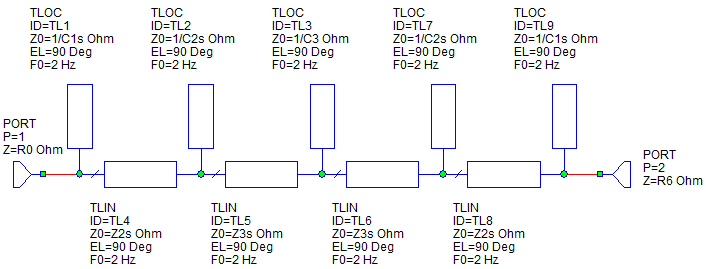
\includegraphics[width=\imagewidth]{images/stripline-kuroda}
    \caption{Resultierende Umwandlung der Schaltung mithilfe der Kuroda-Transformation}
    \label{fig:stripline-kuroda}
\end{figure}

\begin{figure}[h!]
    \centering
    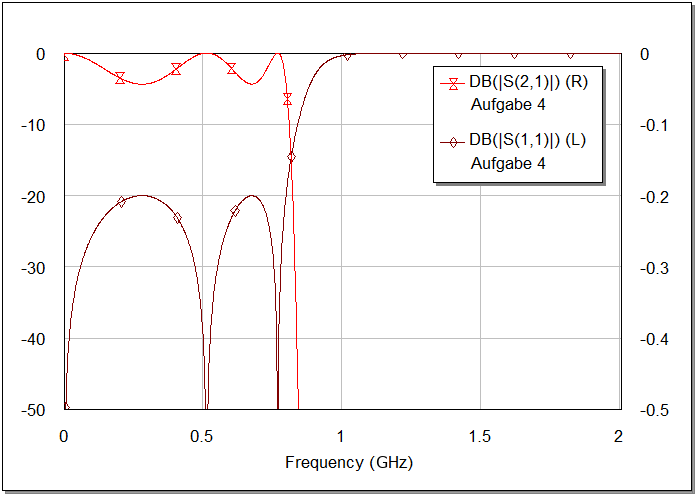
\includegraphics[width=\imagewidth]{images/graph-kuroda}
    \caption{}
    \label{fig:graph-kuroda}
\end{figure}

